\PassOptionsToPackage{unicode=true}{hyperref} % options for packages loaded elsewhere
\PassOptionsToPackage{hyphens}{url}
%
\documentclass[12pt,]{extarticle}
\usepackage{lmodern}
\usepackage{amssymb,amsmath}
\usepackage{ifxetex,ifluatex}
\usepackage{fixltx2e} % provides \textsubscript
\ifnum 0\ifxetex 1\fi\ifluatex 1\fi=0 % if pdftex
  \usepackage[T1]{fontenc}
  \usepackage[utf8]{inputenc}
  \usepackage{textcomp} % provides euro and other symbols
\else % if luatex or xelatex
  \usepackage{unicode-math}
  \defaultfontfeatures{Ligatures=TeX,Scale=MatchLowercase}
\fi
% use upquote if available, for straight quotes in verbatim environments
\IfFileExists{upquote.sty}{\usepackage{upquote}}{}
% use microtype if available
\IfFileExists{microtype.sty}{%
\usepackage[]{microtype}
\UseMicrotypeSet[protrusion]{basicmath} % disable protrusion for tt fonts
}{}
\IfFileExists{parskip.sty}{%
\usepackage{parskip}
}{% else
\setlength{\parindent}{0pt}
\setlength{\parskip}{6pt plus 2pt minus 1pt}
}
\usepackage[colorlinks]{hyperref}
\hypersetup{
            pdftitle={Tutor:Curvas de Nivel},
            pdfauthor={Mariano Harguinteguy, Javier J. Clavijo},
            pdfborder={0 0 0},
            breaklinks=true}
\urlstyle{same}  % don't use monospace font for urls
\usepackage[margin=2.5cm]{geometry}
\usepackage{longtable,booktabs}
% Fix footnotes in tables (requires footnote package)
\IfFileExists{footnote.sty}{\usepackage{footnote}\makesavenoteenv{longtable}}{}
\usepackage{graphicx,grffile}
\makeatletter
\def\maxwidth{\ifdim\Gin@nat@width>\linewidth\linewidth\else\Gin@nat@width\fi}
\def\maxheight{\ifdim\Gin@nat@height>\textheight\textheight\else\Gin@nat@height\fi}
\makeatother
% Scale images if necessary, so that they will not overflow the page
% margins by default, and it is still possible to overwrite the defaults
% using explicit options in \includegraphics[width, height, ...]{}
\setkeys{Gin}{width=\maxwidth,height=\maxheight,keepaspectratio}
\setlength{\emergencystretch}{3em}  % prevent overfull lines
\providecommand{\tightlist}{%
  \setlength{\itemsep}{0pt}\setlength{\parskip}{0pt}}
\setcounter{secnumdepth}{0}
% Redefines (sub)paragraphs to behave more like sections
\ifx\paragraph\undefined\else
\let\oldparagraph\paragraph
\renewcommand{\paragraph}[1]{\oldparagraph{#1}\mbox{}}
\fi
\ifx\subparagraph\undefined\else
\let\oldsubparagraph\subparagraph
\renewcommand{\subparagraph}[1]{\oldsubparagraph{#1}\mbox{}}
\fi

% set default figure placement to htbp
\makeatletter
\def\fps@figure{htbp}
\makeatother

\usepackage{wrapfig}
\usepackage{polyglossia}
\setmainlanguage{spanish}
\usepackage[dvipsnames]{xcolor}
\setlength{\fboxrule}{2pt}

\begin{document}

\hypertarget{extraer-curvas-de-nivel-de-un-modelo-raster-con-qgis}{%
\section{Extraer curvas de nivel de un modelo raster con
QGis}\label{extraer-curvas-de-nivel-de-un-modelo-raster-con-qgis}}

En este tutorial, partiendo de un archivo raster en formato .tiff del
modelo digital de elevaciones PALSAR, que contiene información de
elevaciones de terreno, generaremos curvas de nivel. En otras palabras,
vectorizaremos información altimétrica del terreno que viene dada en
formato raster. Para ello utilizaremos el software QGis.

Los archivos del tipo GeoTiff, como los utilizados en nuestro caso,
pueden contener distintos tipos de información. Sin embargo, su
característica distintiva es que este formato soporta agregar
información de referencia geográfica a la información púramente raster
contenida en él.

\hypertarget{aclaraciuxf3n-sobre-el-funcionamiento-de-qgis}{%
\subsection{Aclaración sobre el Funcionamiento de
QGis}\label{aclaraciuxf3n-sobre-el-funcionamiento-de-qgis}}

Los software del tipo GIS --sistema de información geográfica-- es
específico para el manejo de información georreferenciada. Su principal
capacidad es la de interpretar coordenadas almacenadas en distintos
tipos de archivos y mostrarlas en forma geográficamente correcta,
teniendo en cuenta los distintos sistemas de referencia y de
representación en los que están expresadas las coordenadas.

En este ejemplo, utilizaremos QGis a modo de herramienta de
procesamiento, ingresando nuestra información ráster en una capa, y
sometiendo a la misma a distintos procesos en forma secuencial,
extrayendo en cada caso una nueva capa modificada. De esta manera el
archivo ingresado no se modifica en el proceso, sino que se crean
sucesivas capas temporales que, en caso de ser de interes, deben
guardarse como nuevos archivos, \textbf{antes de cerrar el programa}.

Aclaramos que, aún cuando se grabe el proyecto en QGis, si no se graba
cada capa temporal a alguna ruta conocida, no será posible recuperar
dichas capas al volver a abrir el proyecto.

\hypertarget{paso-1-cargar-archivo-raster}{%
\subsection{Paso 1: Cargar archivo
raster}\label{paso-1-cargar-archivo-raster}}

Partiendo del archivo .tiff descargado, el primer paso consiste en
cargarlo en una nueva capa raster. En el menu superior, la opción a
utilizar para ello es la que sigue.

\begin{quote}
Capas \textgreater{} Añadir capa \textgreater{} Añadir capa ráster.
\end{quote}

\begin{figure}
\centering
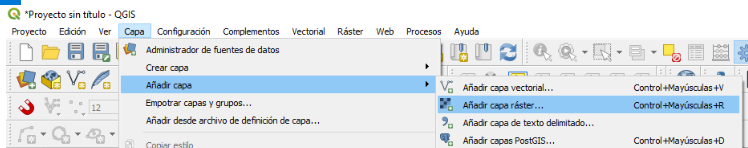
\includegraphics[width=5.90556in,height=1.16875in]{../img/image1.png}
\caption{Menú para añadir capa raster.}
\end{figure}

Para elegir el archivo desado, en el dialogo desplegado se hace clic en
el ícono ``\ldots{}'', se busca la ruta correspondiente, presionando
luego añadir.

Una vez realizado este paso veremos añadirse al panel de capas --listado
en la parte inferior izquierda de la pantalla-- la nueva capa.

\hypertarget{paso-2-recortar-archivo-raster.}{%
\subsection{Paso 2: Recortar archivo
raster.}\label{paso-2-recortar-archivo-raster.}}

El paso que sigue no es estricamente obligatorio, pero aporta a obtener
un archivo más fácil de procesar.

Debe notarse que los límites del modelo y la zona de trabajo deseada no
son necesariamente coincidentes, de manera tal que resulta útil recortar
el ráster al area de interés. En el caso que nos ocupa, el area de
interés que queda definida por los límites de la carta elegida para el
trabajo práctico. Las coordenadas del límite las expresaremos en
coordenadas geográficas, con grado y decimal de grado, porque es éste el
sistema de referencia utilizado en el archivo raster que manejamos --
ver \href{https://epsg.io/4326}{epsg:4326} --.

Para el trabajo que realizaremos, la carta fue provista en formato jpeg,
es decír que es una imagen sin información de georreferenciación. Sin
embargo, los límites de la carta estan expresados explícitamente en los
vértices inferior izquierdo y superior derecho de la representación, tal
como se ve en las figuras 2 y 3.

\begin{figure}
\centering
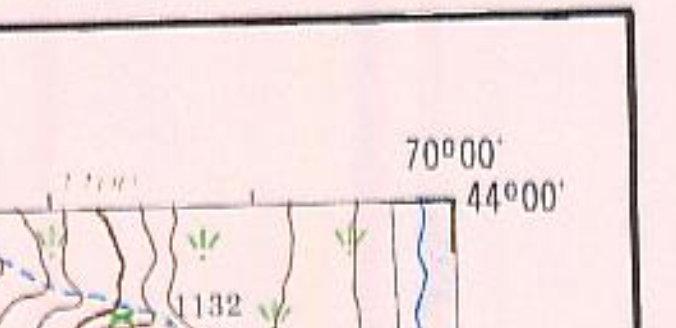
\includegraphics[width=2.48958in,height=1.2079in]{../img/image2.png}
\caption{Vertice superior de la carta}
\end{figure}

\begin{figure}
\centering
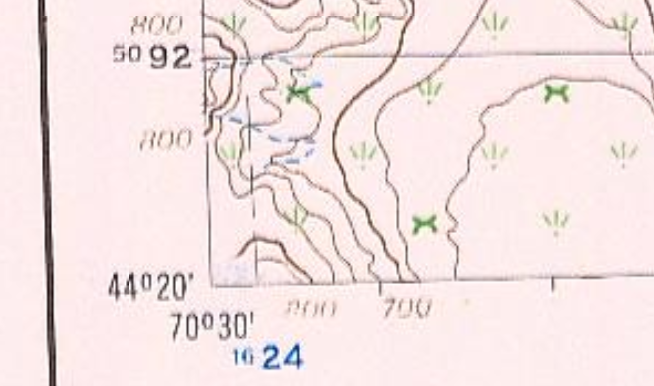
\includegraphics[width=1.97676in,height=1.16667in]{../img/image3.png}
\caption{Vertice inferior de la carta}
\end{figure}

\begin{quote}
Es importante en este momento notar que el sistema de coordenadas que
estamos utilizado en QGis es como ya dijimos epsg:4326, y podemos
verificarlo en la esquina inferior derecha, este sistema es simplemente
la asignación de y=longitud , x=latitud en grados.
\end{quote}

La herramienta que utilizaremos para cortar los datos se encuentra en la
caja de herramientas de procesos, utilizando el buscador que aparece en
la parte derecha de la pantalla. El nombre de la herramienta es ``cortar
ráster por extensión''

\begin{figure}
\centering
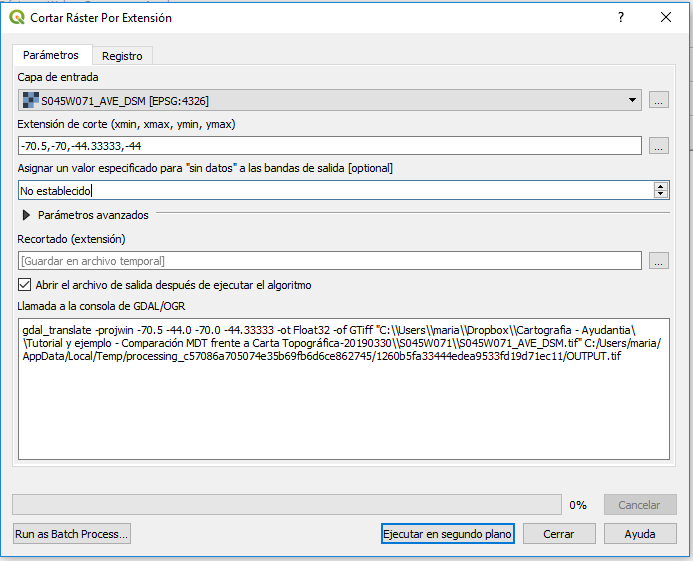
\includegraphics[width=5.90556in,height=4.78056in]{../img/image4.png}
\caption{Dialogo de ``cortar raster por extensión''}
\end{figure}

Los datos requeridos por esta herramienta son el nombre de la capa a
recortar y los limites expresados como máximos y mínimos de x e y,
interpertados como longitud y latitud respectivamente. Es importante
recordar que las coordenadas geográficas oeste y sur tienen signo
negativo.

Una vez realizado este paso, estaremos en condiciones de generar las
curvas de nivel. En caso de saltearlo y utilizar el raster completo para
la generación de curvas, el tiempo de procesamiento se verá aumentado.

\hypertarget{paso-3-generacion-de-curvas-de-nivel}{%
\subsection{Paso 3: Generacion de curvas de
nivel:}\label{paso-3-generacion-de-curvas-de-nivel}}

Para el tercer paso utilizaremos, nuevamente de la caja de herramienta
de procesos, la herramienta que aparece como ``curvas de nivel''.

Los datos requeridos son la capa de entrada, la equidistancia y un
nombre de atributo para asignar la altura correspondiente a cada línea.
La equidistancia deberá elegirse en funcion de las características de la
zona de trabajo, teniendo en cuenta que debemos lograr curvas que
permitan apreciar los picos de altura y sean comparables con las curvas
de la carta. El nombre de atributo es arbitrario y puede dejarse el
valor que viene por defecto

Es posible que en este paso se generen capas innecesarias, producto de
elegir valores no adecuados de equidistancia.

\textbf{Para eliminar una capa añadida a QGis}, se debe haciendo clic
derecho sobre el nombre de capa \textgreater{} Remove layer

\hypertarget{paso-4-guardar-y-reproyectar-el-archivo-de-curvas-de-nivel.}{%
\subsection{Paso 4: Guardar y reproyectar el archivo de curvas de
nivel.}\label{paso-4-guardar-y-reproyectar-el-archivo-de-curvas-de-nivel.}}

Una vez finalizado el proceso de vectorizacion, el paso que sigue será
la exportación de la capa en un formato conveniente, y la reproyección
del mismo a un sistema de coordenadas adecuado para la zona de trabajo.

\begin{quote}
\textbf{Para exportar una capa desde Qgis}, en el panel de capas hacemos
Clic derecho sobre capa \textgreater{} Exportar \textgreater{} Save
features as

y debemos

\begin{itemize}
\item
  Elegir formato de archivo: por ejemplo .dxf de manera que sea
  compatible con AutoCad.
\item
  Elegir nombre y ubicación del archivo: Seleccionar una ubicación
  válida para guardar el archivo, haciendo clic sobre ``\ldots{}'' a la
  derecha de ``Nombre de archivo''.
\item
  Elegir el SRC correspondiente. En el ejemplo Posgar07 con el número de
  faja que corresponda a la carta elegida --ver figura 5--
\end{itemize}
\end{quote}

\begin{figure}
\centering
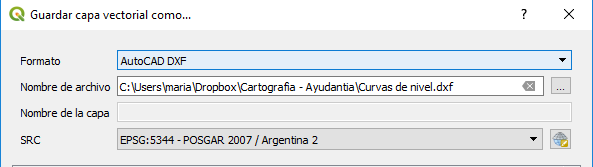
\includegraphics[width=5.90556in,height=1.66319in]{../img/image5.png}
\caption{Dialogo de exportación de capa.}
\end{figure}

\hypertarget{generaciuxf3n-de-curvas-con-gdal-y-ogr-desde-osgeo4w-shell}{%
\section{\texorpdfstring{Generación de Curvas con GDAL y OGR, desde
\emph{OsGeo4w
Shell}}{Generación de Curvas con GDAL y OGR, desde OsGeo4w Shell}}\label{generaciuxf3n-de-curvas-con-gdal-y-ogr-desde-osgeo4w-shell}}

Una forma alternativa para extraer curvas de nivel a partir de un
archivo ráster es utilizar las herramientas de línea de comandos de GDAL
y OGR, accesibles a través de la consola OsGeo4w Shell, que se instala
junto con QGis. El procedimiento a seguir es similar al utilizado para
la extracción QGIS, pero el procesado se hace sin necesidad de observar
las salidas gráficas intermedias.

Para iniciar recomendamos utilizar una ruta fácil de tipear, cercana a
la raiz del disco utilizado -- C:, D:, etc.. --, Por ejemplo:
C:\textbackslash{}Users\textbackslash{}maria\textbackslash{}Documents\textbackslash{}CartaSanMartin

La consola OsGeo4w Shell tiene un comportamiento similar a la línea de
comandos tradicional de windows, a la que se accede con la orden ``cmd''
desde el menú de inicio. Recordamos que en este contexto el clic derecho
funciona como comando de copiar y pegar textos seleccionados en la
consola, como por ejemplo la ruta al archivo.

\hypertarget{paso-1-recortar-el-archivo-raster}{%
\subsection{Paso 1: Recortar el archivo
raster}\label{paso-1-recortar-el-archivo-raster}}

Para empezar debemos abrir la consola, que puede ubicarse desde el
buscador del menú de inicio ingresand en el cuadro de búsqueda
``osgeow4''. Una vez abierta nos moveremos al directorio en el que está
el archivo utilizando el comando
\href{https://www.computerhope.com/cdhlp.htm}{cd}:

C:\textbackslash{}\textgreater{} cd
Users\textbackslash{}maria\textbackslash{}Documents\textbackslash{}CartaSanMartin

La orden que utilizaremos para cortar el archivo raster es
``gdal\_translate'', los parámetros e ingresan en general con un nómbre
de opción precedido de un ``-'' y luego el parámetro de la upcion. Por
ejemplo, la opción -projwin lleva 4 parámetros que son los límites del
recorte a realizar, recorridos en sentido horario comenzando por la
longitud del borde izquierdo.

Para cualquiera de las ordenes a ingresar, si se ingresa el comando sin
parámetros se obtiene la ayuda de uso.

El comando completo para cortar un archivo raster, suponiendo que se
llama ``entrada.tif'' y se quiere obtener un archivo cortado
``salida.tif'', es:

\begin{verbatim}
gdal_translate -projwin x_izq y_arriba x_der y_abajo ^
               -of "GTiff" entrada.tif salida.tif
\end{verbatim}

Los parámetros ingresados en esta caso son

\begin{itemize}
\item
  \textbf{gdal\_translate -projwin:} Comando de recorte.
\item
  \textbf{x\_izq y\_arriba x\_der y\_abajo:} Limites del recorte x min,
  y max, x max, y min, sabiendo que las coordenadas se expresan en:
  latitud=y, longitud=x.
\item
  \textbf{-of:} formato de salida.
\item
  Nombres de archivo de entrada y salida.
\end{itemize}

Como ejemplo, para la carta de San Martín, el recorte queda

\begin{verbatim}
gdal_translate -projwin -70.33 -44 -70 -44.5 -of "GTiff" ^
               S045W071_AVE_DSM.tif recortado.tif
\end{verbatim}

\hypertarget{paso-2-generaciuxf3n-de-curvas-de-nivel}{%
\subsection{Paso 2: Generación de curvas de
nivel}\label{paso-2-generaciuxf3n-de-curvas-de-nivel}}

A partir de la imagen recortada, en el segundo paso se extraerá un
archivo vectorial con curvas de nivel.

El comando a utilizar en este caso es ``gdal\_contour'', cuyo uso para
nuestro caso es como sigue.

\begin{verbatim}
gdal_contour -a elev -i 100 archivoentrada.tif -f "geojson" ^
             archivosalida.geojson
\end{verbatim}

Donde kas opciones utilizadas fueron

\begin{itemize}
\item
  \textbf{-a:} nombre del atributo del ráster a utilizar.
\item
  \textbf{-i:} Equidistancia.
\item
  \textbf{-f:} formato de archivo de salida.
\end{itemize}

El mismo ejemplo, con la carta da General San Martin, partiendo del
archivo recortado queda

\begin{verbatim}
gdal_contour -a elev -i 100 recortado.tif -f "geojson" ^
             CurvasSanMartin.geojson
\end{verbatim}

Una vez finalizado el proceso, podemos observar en el explorador de
archivos si aparece el archivo creado --figura 6--. Esto puede
efectuarse tambien utilizando el comando dir para listar el contenido
del directorio desde la linea de comandos.

\begin{figure}
\centering
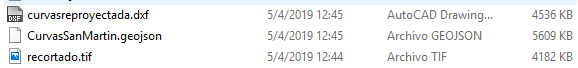
\includegraphics[width=5.91667in,height=0.64236in]{../img/image11.png}
\caption{Archivo creado en la carpeta correspondiente}
\end{figure}

Hacemos notar que el tipo de archivo generado es
\href{http://geojson.org/}{geojson}, podria haberse utilizado cualquier
otro tipo de \href{https://www.gdal.org/ogr_formats.html}{archivo
soportado por ogr},

\hypertarget{paso-3-reproyeccion-de-las-curvas-a-la-faja-correspondiente}{%
\subsection{Paso 3: Reproyeccion de las curvas a la faja
correspondiente}\label{paso-3-reproyeccion-de-las-curvas-a-la-faja-correspondiente}}

El archivo generado previamente, al no haber especificado un cambio de
sistema de coordenadas, está expresado en el mismo sistema del archivo
raster original, el ya mencionado epsg:4326.

Para lograr un resultado que pueda compararse a la carta debemos
utilizar el sistema Gauss Krugger Argentina con la faja oficial
correspondiente.

Para expresar una proyección desde la linea de comandos se utiliza el
lenguaje soportado por la libreria
\href{https://proj4.org/usage/quickstart.html}{proj4}. En nuestro caso
utilizaremos las proj-strings correspondientes a epsg:4326 y a la faja
de Gauss Krugger que corresponda a la carta elegida.

La expresión de la proyeccion EPSG:4326 es siguiente: "+proj=longlat
+datum=WGS84"

\hypertarget{aclaraciuxf3n-fajas-de-gauss-krugger-argentina.}{%
\subsection{Aclaración: Fajas de Gauss Krugger
Argentina.}\label{aclaraciuxf3n-fajas-de-gauss-krugger-argentina.}}

\begin{wrapfigure}{r}{5cm}
\centering
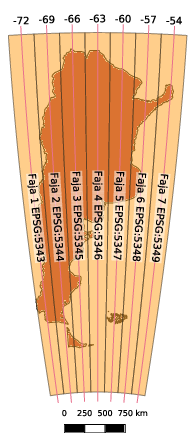
\includegraphics[width=\linewidth]{../img/image12.png}
\caption{Fajas de Gauss-Krugger Argentina}
\end{wrapfigure}

El sistema de proyección cartográfica oficial de la república Argentina,
definido por el instituto geográfico nacional es el sistema Gauss
Krugger, que cuenta con 7 fajas -- o zonas -- diferenciadas.

Para faja, se aplica una proyección cilíndrica transversa con parámetros
distintos. Una faja abarca un ancho de 3° en longitud, 1.5° a cada lado
respecto a un meridiano central, que se encuentra representado en
magnitud verdadera..

Para más información ingresar a la
\href{http://www.ign.gob.ar/NuestrasActividades/ProduccionCartografica/sistemas-de-proyeccion}{página
oficial del IGN}

Los parámetros de cada faja se listan en la tabla que sigue.

\begin{minipage}{10cm}
\begin{longtable}[]{@{}lllccc@{}}
\toprule
Faja & \(\Lambda\) Central & E Origen & \(\varphi\) Origen & N Origen &
Escala\tabularnewline
\midrule
\endhead
1 & -72° & 1.500.000 m & -90° & 0 m & 1\tabularnewline
2 & -69° & 2.500.000 m & -90° & 0 m & 1\tabularnewline
3 & -66° & 3.500.000 m & -90° & 0 m & 1\tabularnewline
4 & -63° & 4.500.000 m & -90° & 0 m & 1\tabularnewline
5 & -60° & 5.500.000 m & -90° & 0 m & 1\tabularnewline
6 & -57° & 6.500.000 m & -90° & 0 m & 1\tabularnewline
7 & -54° & 7.500.000 m & -90° & 0 m & 1\tabularnewline
\bottomrule
\end{longtable}
\end{minipage}

De la tabla anterior se debe identificar la faja correspondiente al área
de trabajo, y modificar los siguientes parámetros para construir la
cadena-proj de la proyección en que se desea adquirir las curvas:

\begin{itemize}
\item
  +lon\_0: meridiano central
\item
  +lat\_0: origen de latitudes
\item
  +x\_0: coordenada este del meridiano central.
\end{itemize}

\hypertarget{continuaciuxf3n-paso-3}{%
\subsection{Continuación Paso 3}\label{continuaciuxf3n-paso-3}}

El comando que se utilizará en este paso es ``ogr2ogr'',

las opciones a utilizar son

\begin{itemize}
\item
  -s\_srs parametros de proyeccion de entrada
\item
  -t\_srs parametros de proyeccion de salida
\item
  -f formato de salida
\item
  -skipfailures para ignorar algunos errores en la creacion del archivo
\end{itemize}

Las cadenas de la proyecciones a utilzar, por ejemplo para una carta en
faja 2 son

\begin{itemize}
\item
  EPSG: 4326 = ``+proj=longlat +datum=WGS84''
\item
  Faja 2 = ``+proj=tmerc +ellps=GRS80 +lat\_0=-90 +lon\_0=-69
  +x\_0=2500000''
\end{itemize}

De manera que la expresión del comando para la reproyectar el archivo de
curvas de nivel obtenido anteriormente en el ejemplo para San Martín es:

\begin{verbatim}
ogr2ogr -s_srs "+proj=longlat +datum=WGS84" ^
   -t_srs "+proj=tmerc +ellps=GRS80 +lat_0=-90 +lon_0=-69 +x_0=2500000"^
   -f "dxf" curvasreproyectada.dxf curvassanmartin.geojson -skipfailures
\end{verbatim}

\hypertarget{ejemplo-completo}{%
\subsection{Ejemplo completo}\label{ejemplo-completo}}

Para ver el ejemplo completo para la carta de San Martín puede
consultarse la figura 8.

\begin{figure}
\centering
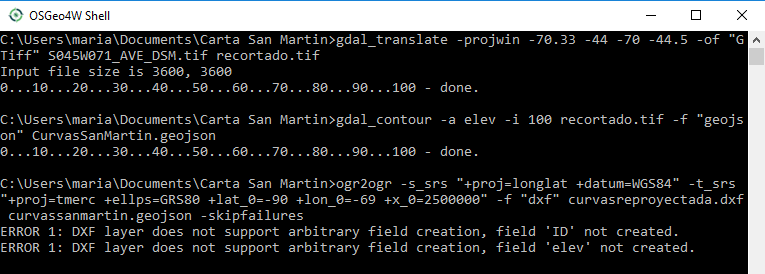
\includegraphics[width=6.38777in,height=2.288in]{../img/image13.png}
\caption{ejemplo para Carta General San Martín}
\end{figure}

La ventaja del procesamiento desde la línea de comantos es la
escalabilidad de la solución, es decir, que en caso de necesitar aplicar
el mismo proceso a un grán numero de imágenes, el mismo puede hacerse en
forma automatizada y sin tenér los problemas de manejo de memoria que
trae el cargar demasiadas capas en simultaneo en el software de GIS que
se utilize.

\end{document}
